% !TeX root = ../main.tex
\chapter{训练}

如 \ref{sec1.1} 节所述,训练模型包括最小化损失 $\mathcal{L}(w)$,它反映了预测器 $f(\cdot;w)$ 在\keyterm{训练集} $\mathcal{D}$ 上的表现。

由于模型通常非常复杂,并且其表现与损失最小化程度直接相关,因此这里的最小化是一个关键挑战,涉及计算和数学难题。

\section{损失}

公式 \ref{eq1.1} 中的\keyterm{均方误差}示例是用于预测连续值的标准损失。

在密度建模中,标准损失是数据的似然度。如果 $f(x;w)$ 被解释为归一化的对数概率或对数密度,那么损失就是其值在训练样本上的总和的相反数,这对应于数据集的似然度。

\subsubsection*{交叉熵}

对于\keyterm{分类},通常的策略是模型的输出是一个向量,其中每个类别 $y$ 对应一个分量 $f(x;w)_y$,这被解释为非归一化概率的对数或 \keyterm{logit}。

如果 $X$ 为输入信号,$Y$ 为要预测的类别,我们可以根据 $f$ 计算\keyterm{后验概率}估计:
\[\hat{P}(Y=y \mid X=x) = \frac{\exp f(x;w)_y}{\sum_{z}\exp f(x;w)_z}\]
该表达式通常称为 logits 的 \keyterm{softmax},或更准确地说,称为 \keyterm{softargmax}。

为了与这种解释保持一致,模型应该被训练来最大化真实类别的概率,因此要最小化交叉熵,其表达式如下:
\begin{align*}
    \mathcal{L}_{ce}(w) &= -\frac{1}{N}\sum_{n=1}^{N} \log \hat{P}(Y=y_n \mid X=x_n) \\
    &= \frac{1}{N}\sum_{n=1}^{N} \underbrace{-\log \frac{\exp f(x_n;w)_{y_n}}{\sum_{z}\exp f(x_n;w)_z}}_{L_{ce}(f(x_n;w),y_n)}
\end{align*}

\subsubsection*{对比损失}

在某些设置中,即使要预测的值是连续的,监督也会采取排名约束的形式。这种情况的典型领域是\keyterm{度量学习},其目标是学习样本之间距离的度量,使得来自某个语义类别的样本 $x_a$ 与同一类别中的任意样本 $x_b$ 之间的距离都比来自另一个类别的任意样本 $x_c$ 之间的距离更近。例如,$x_a$ 和 $x_b$ 可以是某个人的两张照片,而 $x_c$ 则是另一个人的照片。

这种情况的标准方法是最小化\keyterm{对比损失},在这种情况下,例如,三元组 $(x_a,x_b,x_c)$,满足 $y_a = y_b \ne y_c$,求和
\[\max(0,1-f(x_a,x_c;w)+f(x_a,x_b;w))\]
除非 $f(x_a,x_c;w) \ge 1+f(x_a,x_b;w)$,否则该量将严格为正。

\subsubsection*{工程化损失}

通常,在训练期间最小化的损失并不是最终想要优化的实际量,而是一个代理量,是为了让找到最佳模型参数更为容易。例如,尽管实际的性能度量是分类错误率,但交叉熵是分类的标准损失,因为后者没有提供信息梯度,这是我们将在 \ref{sec3.3} 节中看到的关键要求。

还可以在损失中添加取决于模型本身的可训练参数项,以支持某些配置。

例如,\keyterm{权重衰减}正则化包括向损失中增加一个与参数平方和成比例的项。这可以被解释为在参数上施加了一个高斯贝叶斯先验,它偏好较小的值,从而减少了数据的影响。这会降低其在训练集上的表现,但会减少训练表现与新的、未见过的数据上的表现之间的差距。

\section{自回归模型}

自回归模型是一类关键方法,特别适用于处理自然语言处理和计算机视觉中的离散序列。

\subsubsection*{概率的链式法则}

这些模型使用概率论中的\keyterm{链式法则}:
\begin{align*}
    P(&X_1 = x_1,X_2 = x_2,\dots,X_T = x_T) = \\
    &P(X_1 = x_1) \\
    \times &P(X_2 = x_2 \mid X_1 = x_1) \\
    &\dots \\
    \times &P(X_T = x_T \mid X_1 = x_1,\dots,X_{T-1} = x_{T-1})
\end{align*}
尽管这种分解对于任何类型的随机序列都有效,但当感兴趣的信号是来自有限\keyterm{词汇表} $\{1, \dots ,K\}$ 的 \keyterm{Token} 序列时,它特别有效。

按照约定,附加 Token $\emptyset$ 代表``未知''量,我们可以将事件 ${X_1 = x_1,\dots,X_t = x_t}$ 表示为向量 $(x_1,\dots,x_t,\emptyset,\dots,\emptyset)$。则模型
\[f : \{\emptyset,1,\dots,K\}^T \to \mathbb{R}^K\]
在给定这样的输入的情况下计算与
\[\hat{P}(X_t \mid X_1 = x_1,\dots,X_{t-1} = x_{t-1})\]
相对应的 $K$ 个 \keyterm{logits} 的向量 $l_t$,允许在给定先前 Token 的情况下对一个 Token 进行采样。

链式法则确保在给定先前采样的 $x_1,\dots,x_{t-1}$ 的情况下,通过一次次地对第 $T$ 个 Token $x_t$ 进行采样,我们能够得到一个遵循联合分布的序列。这是一个\keyterm{自回归}生成模型。

训练这样的模型可以通过最小化训练序列和时间帧上的\keyterm{交叉熵损失}
\[Lce\big(f(x_1,\dots,x_{t-1},\emptyset,\dots,\emptyset;w),x_t\big)\]
之和来完成,这在形式上等同于最大化真实 $x_t$ 的似然。

传统上监测的值不是交叉熵本身,而是\keyterm[困惑度]{困惑度(Perplexity)},其定义为交叉熵的指数。它对应于具有相同熵的均匀分布的值的数量,这通常更易于解释。

\subsubsection*{因果模型}

\begin{figure}
    \centering
    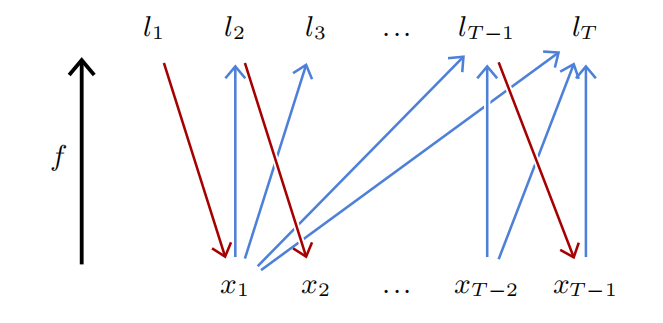
\includegraphics[width=0.9\textwidth]{fig/fig3.1.png}
    \caption[因果自回归模型]{如果输入序列的一个时间帧 $x_t$ 调节预测的 logits $l_s$ 只在 $s > t$ 时才有效,如蓝色箭头所示,则自回归模型 $f$ 是因果模型。这允许在训练期间一次性计算所有时间帧的分布。然而,在采样过程中,$l_t$ 和 $x_t$ 是顺序计算的,后者是用前者采样的,如红色箭头所示。}
    \label{fig3.1}
\end{figure}

\subsubsection*{Tokenizer}

\section{梯度下降}\label{sec3.3}

\subsubsection*{学习率}

\subsubsection*{随机梯度下降}

\section{反向传播}

\subsubsection*{正向和反向传递}

\subsubsection*{资源利用}

\subsubsection*{梯度消失}

\section{深度值}\label{sec3.6}

\section{训练协议}\label{sec3.7}

\section{规模的好处}